\chapter{وصف نظام كيميائي: التقدم والنشاطيات وخارج التفاعل وثابت التوازن}\label{ch:b1:extent-q-and-k}

يُغذّى مصنع هيدروجين بالغاز الطبيعي وبخار الماء في أنابيب مسخّنة حتى الاحمرار؛
فلا يخرج منها هيدروجين نقي أبدًا، بل خليط من الهيدروجين وأحادي أكسيد
الكربون وثنائي أكسيد الكربون والميثان الذي لم يتفاعل وبخار الماء، ويجب على
المهندسين أن يعرفوا نسبه قبل أن يصمموا الوحدة التالية. والتنبؤ
بالتركيب الذي يغادر المفاعل --- أي بالحالة النهائية لنظام
كيميائي --- هو موضوع هذا الفصل. ويحتاج ذلك إلى وصف دقيق
للنظام (متغيراته وتركيبه)، وإلى عدد واحد
يقيس إلى أي حد مضى التفاعل (التقدم)، وإلى القانون
الذي يبيّن أين يتوقف التفاعل (ثابت التوازن).
وتُستعمل هذه الأدوات في كل الفصول اللاحقة عن المحاليل.

\begin{recall}
تتبّع الكتاب الأول (الصف العاشر) تفاعلًا بجدول التقدم وعيّن
\omterm{def:b1:extent-q-and-k:max-extent}{المتفاعل المحدِّد}؛ وقدّم الكتاب الأول (الصف الثاني عشر) \omterm{def:b1:extent-q-and-k:quotient}{خارج التفاعل}
$Q$ وثابت التوازن $K$ لتفاعل غير تام. ونستعمل من
الفيزياء قانون الغاز المثالي $pV = nRT$، مع $R =
\qty{8.314}{J/(mol.K)}$.
\end{recall}

\begin{omfigure}
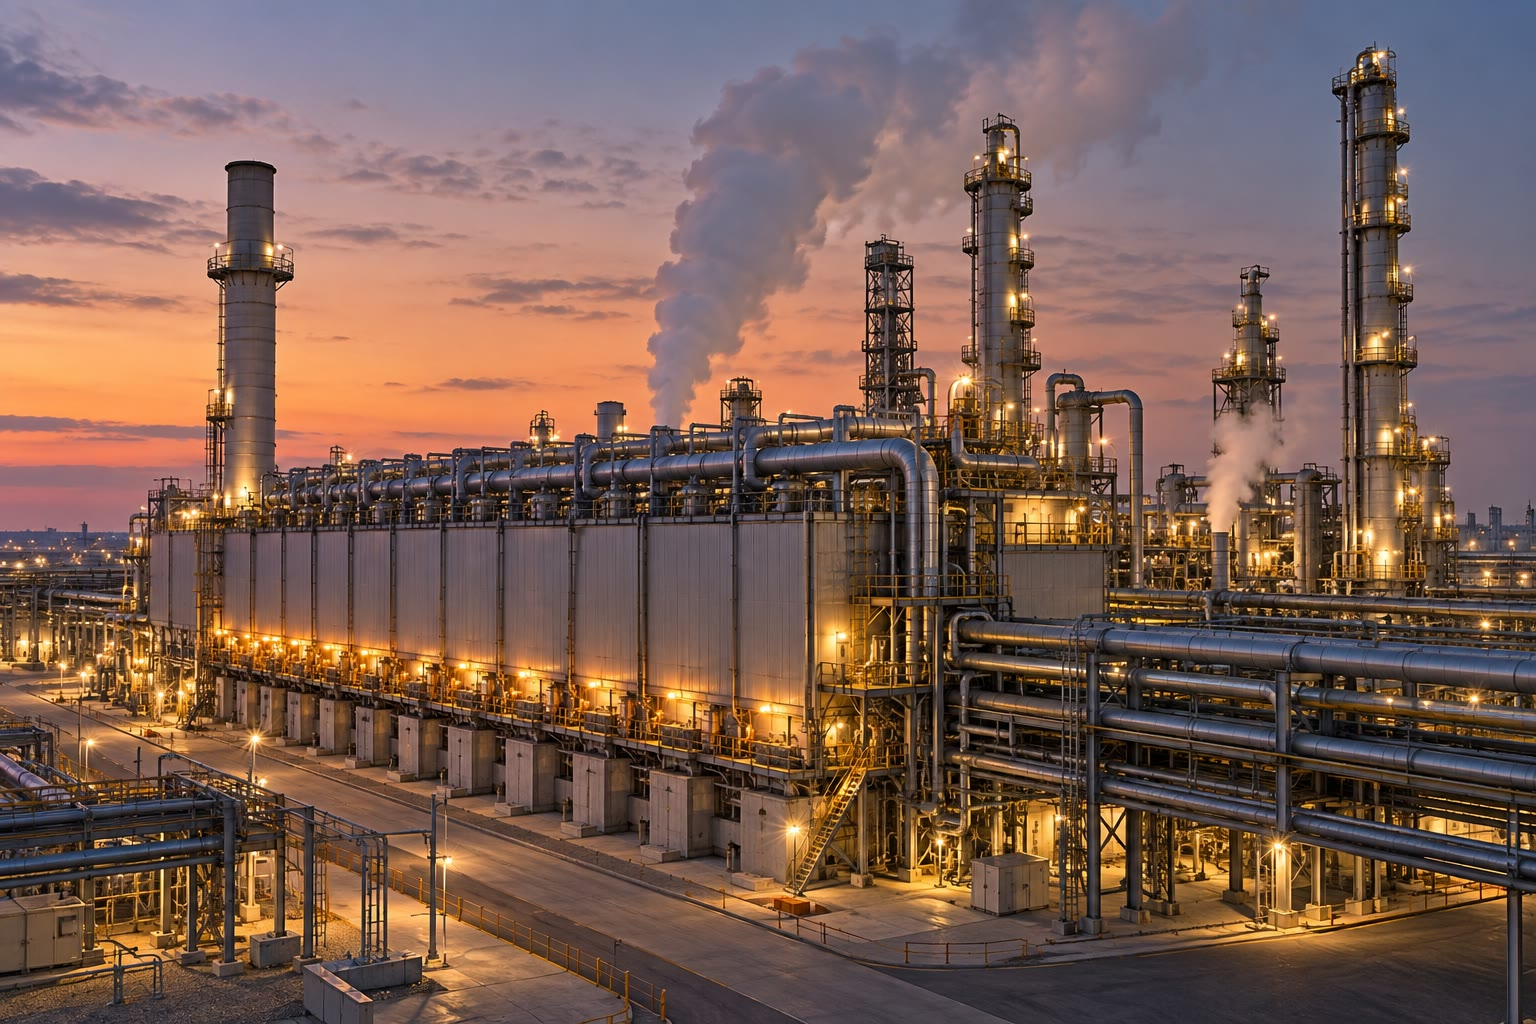
\includegraphics[width=0.6\linewidth]{images/book2/ai/b1-07-hydrogen-plant.jpg}

{\small مصنع هيدروجين عند الغسق. يتفاعل الغاز الطبيعي وبخار الماء في
فرن الإصلاح الطويل؛ ويحوّل مفاعل ثانٍ أحادي أكسيد الكربون؛ والتركيب
عند المخرج حالة نهائية من النوع الذي يُحسب في هذا
الفصل.}
\end{omfigure}

\section{وصف نظام}

\begin{definition}[النظام، الطور]\label{def:b1:extent-q-and-k:system}
\emph{النظام الفيزيائي الكيميائي}\index{نظام فيزيائي كيميائي} هو
المادة المحتواة في منطقة مختارة من الفضاء، والباقي هو
محيطه. ويكون \emph{نظامًا مغلقًا}\index{نظام مغلق} إذا لم
يتبادل مادة مع المحيط (وقد يتبادل طاقة).
و\emph{الطور}\index{طور} جزء من النظام تتغير فيه \omterm{def:b1:extent-q-and-k:variables}{المتغيرات
المكثفة} تغيرًا متصلًا: فخليط الغازات طور واحد، والسائلان غير \omterm{def:b1:intermolecular-forces-solvents:miscibility}{القابلين للامتزاج}
طوران، وكل جسم صلب طور قائم بذاته.
\end{definition}

\begin{definition}[المتغيرات المكثفة والممتدة]\label{def:b1:extent-q-and-k:variables}
يكون متغير الحالة \emph{ممتدًا}\index{متغير ممتد} إذا كان
متناسبًا مع حجم النظام (الكتلة، والحجم، وكمية
المادة) و\emph{مكثفًا}\index{متغير مكثف} إذا لم يكن كذلك
(درجة الحرارة، والضغط، والتركيز، والكتلة الحجمية، \omterm{def:b1:extent-q-and-k:composition}{والكسر المولي}). ونسبة
متغيرين ممتدين متغير مكثف.
\end{definition}

\begin{definition}[متغيرات التركيب]\label{def:b1:extent-q-and-k:composition}
من أجل مكوّن $i$ \omterm{def:b1:extent-q-and-k:system}{لطور} يحوي الكميات $n_j$ من كل
مكوّناته:
\begin{itemize}
  \item \emph{كسره المولي}\index{كسر مولي} هو $x_i = n_i/\sum_j
        n_j$، و\emph{كسره الكتلي}\index{كسر كتلي} $w_i =
        m_i/\sum_j m_j$؛ وكلاهما بين 0 و1 ومجموع كل منهما 1؛
  \item في محلول حجمه $V$، يكون \emph{تركيزه
        المولي}\index{تركيز مولي} $c_i = [i] = n_i/V$،
        بالوحدة \unit{mol/L}؛
  \item في خليط غازي ضغطه الكلي $p$، يكون \emph{ضغطه
        الجزئي}\index{ضغط جزئي} $p_i = x_i\,p$.
\end{itemize}
\end{definition}

\begin{proposition}[الضغوط الجزئية للغازات المثالية]\label{prop:b1:extent-q-and-k:dalton}
في خليط من غازات مثالية حجمه $V$ عند درجة الحرارة $T$، يكون
\omterm{def:b1:extent-q-and-k:composition}{الضغط الجزئي} لمكوّن هو الضغط الذي يمارسه لو كان وحده في
الحجم كله، $p_i = n_iRT/V$، ومجموع \omterm{def:b1:extent-q-and-k:composition}{الضغوط الجزئية} يساوي
الضغط الكلي: $\sum_i p_i = p$.
\end{proposition}

\begin{proof}
من أجل الخليط $pV = (\sum_j n_j)RT$، فيكون $p_i = x_i p = \frac{n_i}{\sum_j
n_j}\cdot\frac{(\sum_j n_j)RT}{V} = \frac{n_iRT}{V}$، و$\sum_i x_i = 1$
يعطي $\sum_i p_i = p$.
\end{proof}

\begin{example}[الهواء]\label{ex:b1:extent-q-and-k:air}
يحوي الهواء الجاف، حجمًا (أي كميةَ مادة، في الغازات المثالية)،
78.08\,\% من ثنائي النيتروجين، و20.95\,\% من ثنائي الأكسجين و0.93\,\% من الأرغون. وتحت
\qty{1.013}{bar} يكون \omterm{def:b1:extent-q-and-k:composition}{الضغط الجزئي} لثنائي الأكسجين $0.2095 \times
1.013 = \qty{0.212}{bar}$؛ وعلى جبل يبلغ فيه الضغط
\qty{0.70}{bar} ينخفض إلى \qty{0.147}{bar}، مع أن التركيب
هو نفسه.
% ledger: air:N2, air:O2, air:Ar, const:atm
\end{example}

\section{تقدم التفاعل}

\begin{definition}[الأعداد الستوكيومترية، التقدم]\label{def:b1:extent-q-and-k:extent}
يُكتب التفاعل $0 = \sum_i \nu_i\,\mathrm{A}_i$، حيث يكون
\emph{العدد الستوكيومتري}\index{عدد ستوكيومتري} $\nu_i$
للنوع $\mathrm{A}_i$ سالبًا للمتفاعل وموجبًا
للناتج: ففي \ce{N2 + 3H2 -> 2NH3}، $\nu(\ce{N2}) = -1$، $\nu(\ce{H2}) = -3$،
$\nu(\ce{NH3}) = +2$. وفي \omterm{def:b1:extent-q-and-k:system}{نظام مغلق} لا يجري فيه إلا هذا التفاعل،
تتغير الكميات وفق
\[
  n_i = n_{i,0} + \nu_i\,\xi ,
\]
وهذا يعرّف \emph{تقدم التفاعل}\index{تقدم التفاعل}
$\xi$ (بالمول)، المعدوم في البداية والواحد لكل الأنواع.
\end{definition}

\begin{definition}[التقدم الأقصى، المتفاعل المحدِّد]\label{def:b1:extent-q-and-k:max-extent}
\emph{التقدم الأقصى}\index{تقدم أقصى} $\xi_{\max}$ هو أكبر
قيمة للمقدار $\xi$ لا تكون عندها أي كمية سالبة: $\xi_{\max} = \min_{\nu_i <
0} n_{i,0}/|\nu_i|$. والمتفاعل الذي يبلغ الصفر عند $\xi_{\max}$ هو
\emph{المتفاعل المحدِّد}\index{متفاعل محدد}. وحين يمكن أن يكون
التقدم سالبًا أيضًا (التفاعل العكسي)، يكون $\xi_{\min} = -\min_{\nu_i > 0}
n_{i,0}/\nu_i$.
\end{definition}

\begin{method}[جدول التقدم]\label{met:b1:extent-q-and-k:progress-table}
لتتبّع تفاعل في \omterm{def:b1:extent-q-and-k:system}{نظام مغلق}:
\begin{enumerate}
  \item اكتب المعادلة الموزونة، وتحتها عمودًا لكل نوع؛
  \item السطر الأول: الكميات الابتدائية $n_{i,0}$؛
  \item السطر الثاني: الكميات عند التقدم $\xi$، أي $n_{i,0} + \nu_i\xi$؛
  \item للغازات أضف عمودًا للكمية الكلية $n_{\text{كلية}}(\xi)$؛
  \item احسب $\xi_{\max}$ (و$\xi_{\min}$) وعيّن \omterm{def:b1:extent-q-and-k:max-extent}{المتفاعل
        المحدِّد}؛
  \item السطر الأخير: الكميات النهائية، عند التقدم النهائي $\xi_f$ (الذي
        يُستخرج من شرط التوازن، أو يساوي $\xi_{\max}$ إن كان
        التفاعل تامًا).
\end{enumerate}
\end{method}

\begin{example}[تخليق الأمونيا]\label{ex:b1:extent-q-and-k:ammonia}
انطلاقًا من \qty{2.0}{mol} من \ce{N2} و\qty{3.0}{mol} من \ce{H2}:
\begin{center}
\begin{tabular}{lcccc}
\hline
 & \ce{N2} & \ce{3H2} & \ce{2NH3} & المجموع \\
\hline
الحالة الابتدائية & 2.0 & 3.0 & 0 & 5.0 \\
عند التقدم $\xi$ & $2.0 - \xi$ & $3.0 - 3\xi$ & $2\xi$ & $5.0 - 2\xi$ \\
\hline
\end{tabular}
\end{center}
$\xi_{\max} = \min(2.0/1,\ 3.0/3) = \qty{1.0}{mol}$: فثنائي الهيدروجين هو المحدِّد.
ولو كان التفاعل تامًا لاحتوت الحالة النهائية على \qty{1.0}{mol} من
\ce{N2} و\qty{2.0}{mol} من \ce{NH3}.
\end{example}

\begin{definition}[نسبة التقدم النهائي، المردود]\label{def:b1:extent-q-and-k:fractional-extent}
\emph{نسبة التقدم النهائي}\index{نسبة التقدم النهائي} لتفاعل
هي $\tau = \xi_f/\xi_{\max}$، بين 0 و1. وفي التخليق يكون
\emph{مردود}\index{مردود} ناتجٍ نسبةَ الكمية المحصَّلة
إلى الكمية التي كان \omterm{def:b1:extent-q-and-k:max-extent}{المتفاعل المحدِّد} سيعطيها لو كان التفاعل
تامًا؛ وإذا لم يُفقد شيء من الناتج أثناء عزله، كان مساويًا للنسبة $\tau$.
\end{definition}

\section{النشاطيات}

\begin{definition}[الحالة القياسية، النشاطية]\label{def:b1:extent-q-and-k:activity}
\emph{نشاطية}\index{نشاطية} $a_i$ نوعٍ عددٌ بلا أبعاد
يقيس، في التعبير عن قوانين التوازن، القدر المتاح
منه؛ وهي تُعرَّف بالنسبة إلى \emph{حالة
قياسية}\index{حالة قياسية}، أي حالة مرجعية عند درجة الحرارة
المعتبرة وتحت الضغط القياسي $p^\circ = \qty{1}{bar}$. وفي
التقريبات المثالية المستعملة في هذا الكتاب:
\begin{itemize}
  \item للغاز، $a_i = p_i/p^\circ$ (والحالة القياسية هي الغاز المثالي
        النقي عند $p^\circ$)؛
  \item لمذاب في محلول مخفف، $a_i = c_i/c^\circ$ مع
        $c^\circ = \qty{1}{mol/L}$؛
  \item لمذيب محلول مخفف، ولجسم صلب نقي أو
        سائل نقي منفرد في طوره، $a_i = 1$.
\end{itemize}
\end{definition}
% ledger: const:pstd

\begin{remark}[المثالي والحقيقي]\label{rem:b1:extent-q-and-k:ideal}
تصح هذه العبارات في الغازات المثالية وفي المحاليل المخففة. أما في
المحاليل المركزة فتتجاذب الأيونات وتتنافر، فتبتعد
\omterm{def:b1:extent-q-and-k:activity}{النشاطية} عن $c_i/c^\circ$؛ وتُدرس التصحيحات، المكتوبة بمعاملات
\omterm{def:b1:extent-q-and-k:activity}{النشاطية}، في مجلد السنة الثانية مع الجهد
الكيميائي. وفي التراكيز المستعملة في هذا الكتاب (دون نحو
\qty{0.1}{mol/L}) تكون العبارات المثالية دقيقة في حدود بضعة في المئة.
\end{remark}

\section{خارج التفاعل وثابت التوازن}

\begin{definition}[خارج التفاعل]\label{def:b1:extent-q-and-k:quotient}
\emph{خارج التفاعل}\index{خارج التفاعل} لتفاعل
$0 = \sum_i \nu_i\,\mathrm{A}_i$ في حالة معطاة للنظام هو
\[
  Q = \prod_i a_i^{\nu_i} ,
\]
أي جداء نشاطيات النواتج مقسومًا على جداء نشاطيات
المتفاعلات، كل منها مرفوعة إلى أس معاملها الستوكيومتري.
\end{definition}

\begin{example}[ثلاثة خوارج]\label{ex:b1:extent-q-and-k:quotients}
من أجل \ce{N2(g) + 3H2(g) <=> 2NH3(g)}: $Q = \dfrac{(p_{\ce{NH3}}/p^\circ)^2}
{(p_{\ce{N2}}/p^\circ)(p_{\ce{H2}}/p^\circ)^3}$. ومن أجل
\ce{CH3COOH(aq) + H2O(l) <=> CH3COO^-(aq) + H3O+(aq)}: $Q =
\dfrac{[\ce{CH3COO-}][\ce{H3O+}]}{[\ce{CH3COOH}]\,c^\circ}$، إذ \omterm{def:b1:extent-q-and-k:activity}{نشاطية}
المذيب 1. ومن أجل \ce{CaCO3(s) <=> CaO(s) + CO2(g)}: $Q =
p_{\ce{CO2}}/p^\circ$، إذ \omterm{def:b1:extent-q-and-k:activity}{نشاطية} الجسمين الصلبين 1.
\end{example}

\begin{definition}[ثابت التوازن القياسي]\label{def:b1:extent-q-and-k:equilibrium-constant}
\emph{ثابت التوازن القياسي}\index{ثابت التوازن القياسي}
$K^\circ$ لتفاعل هو القيمة التي يأخذها \omterm{def:b1:extent-q-and-k:quotient}{خارج
التفاعل} حين يكون النظام في \omterm{def:b1:extent-q-and-k:quantitative}{حالة توازن}. وهو عدد بلا أبعاد
لا يتعلق إلا بالتفاعل وبدرجة الحرارة.
\end{definition}

\begin{theorem}[قانون فعل الكتلة]\label{thm:b1:extent-q-and-k:mass-action}
عند درجة حرارة معطاة، يتطور النظام الذي يمكن أن يجري فيه تفاعل في
الاتجاهين حتى يصير $Q = K^\circ(T)$؛ وعند التوازن، أيًّا كان
التركيب الابتدائي،
\[
  \prod_i a_{i,\text{توازن}}^{\nu_i} = K^\circ(T) .
\]
\end{theorem}
\admitted

\begin{proposition}[اتجاه التطور]\label{prop:b1:extent-q-and-k:direction}
النظام الذي فيه $Q < K^\circ$ يتطور في الاتجاه المباشر (يتزايد
$\xi$)؛ وإذا كان $Q > K^\circ$، تطوّر في الاتجاه المعاكس؛ وإذا كان
$Q = K^\circ$، فهو في \omterm{def:b1:extent-q-and-k:quantitative}{حالة توازن}.
\end{proposition}
\admitted

\begin{remark}[من أين تأتي هذه القوانين]\label{rem:b1:extent-q-and-k:origin}
تنتج العبارتان كلتاهما من المبدأ الثاني للتحريك الحراري، عبر
الطاقة الحرة للتفاعل والجهود الكيميائية للأنواع: ويُستخرج ذلك
في مجلد السنة الثانية، الذي يعطي أيضًا $K^\circ$ من جداول
المعطيات الترموديناميكية ويبيّن كيف يتغير مع درجة الحرارة. أما هنا
فتُستعمل قوانينَ.
\end{remark}

\begin{omfigure}
\begin{tikzpicture}[font=\small, >={Stealth}]
  \draw[->, thick] (0,0) -- (11,0) node[right] {$Q$};
  \draw[thick, omThm] (5.5,0.25) -- (5.5,-0.25) node[below] {$K^\circ$};
  \draw[->, omDef, thick] (1.0,0.55) -- (4.6,0.55);
  \node[above, omDef] at (2.8,0.6) {\foreignlanguage{arabic}{$Q < K^\circ$: في الاتجاه المباشر}};
  \draw[->, omProp, thick] (10.0,0.55) -- (6.4,0.55);
  \node[above, omProp] at (8.2,0.6) {\foreignlanguage{arabic}{$Q > K^\circ$: في الاتجاه المعاكس}};
  \node[below] at (0,-0.1) {0};
\end{tikzpicture}

{\small يتجه الخارج نحو الثابت: فالنظام الذي فيه $Q <
K^\circ$ يكوّن نواتج، والذي فيه $Q > K^\circ$ يستهلكها.}
\end{omfigure}

\begin{proposition}[تركيب الثوابت]\label{prop:b1:extent-q-and-k:combine-k}
إذا كان $K_1^\circ$ و$K_2^\circ$ ثابتي التفاعلين (1) و(2): كان
للتفاعل العكسي للتفاعل (1) الثابت $1/K_1^\circ$؛ وللتفاعل $n \times
(1)$ الثابت $(K_1^\circ)^n$؛ وللمجموع $(1) + (2)$ الثابت $K_1^\circ K_2^\circ$.
\end{proposition}

\begin{proof}
\omterm{def:b1:extent-q-and-k:quotient}{خارج التفاعل} العكسي هو $\prod a_i^{-\nu_i} = 1/Q_1$؛ وخارج
$n \times (1)$ هو $\prod a_i^{n\nu_i} = Q_1^n$؛ وخارج المجموع هو
$\prod a_i^{\nu_{i,1} + \nu_{i,2}} = Q_1 Q_2$. وبكتابة هذه المتطابقات عند
التوازن، حيث يساوي كل خارج ثابته، نحصل على النتيجة.
\end{proof}

\begin{proposition}[حالة توازن واحدة]\label{prop:b1:extent-q-and-k:q-monotone}
من أجل تفاعل واحد في \omterm{def:b1:extent-q-and-k:system}{نظام مغلق} عند درجة حرارة ثابتة (وبحجم ثابت أو ضغط
ثابت في الغازات)، يكون الخارج $Q(\xi)$ دالة متزايدة
تمامًا في $\xi$ على $(\xi_{\min}, \xi_{\max})$، تنتقل من 0
إلى $+\infty$ ما دام لا يشارك أي نوع ثابت \omterm{def:b1:extent-q-and-k:activity}{النشاطية}. فيكون
للمعادلة $Q(\xi) = K^\circ$ حل واحد بالضبط في هذه
الفترة.
\end{proposition}

\begin{proof}
لنأخذ تفاعلًا في محلول، $Q(\xi) = \prod_i (n_{i,0} + \nu_i\xi)^{\nu_i}
\times \text{ثابت}$. ومشتقته اللوغاريتمية
\[
  \frac{\dd \ln Q}{\dd \xi} = \sum_i \frac{\nu_i^2}{n_{i,0} + \nu_i \xi}
  > 0 ,
\]
وكل حد فيها موجب حيث تكون الكميات كلها موجبة. وعندما $\xi \to \xi_{\max}$ تؤول
كمية متفاعل في مقام إلى 0 فيؤول $Q \to +\infty$؛ وعندما $\xi
\to \xi_{\min}$ تؤول كمية ناتج إلى 0 فيؤول $Q \to 0$. والدالة المتصلة
المتزايدة من 0 إلى $+\infty$ تأخذ القيمة $K^\circ$ مرة واحدة.
(وفي الغازات تحت ضغط ثابت تتغير الكمية الكلية أيضًا؛ وتبقى النتيجة
صحيحة، كما يمكن التحقق في كل حالة.)
\end{proof}

\section{الحالات النهائية}

\begin{definition}[حالة التوازن، التفاعل الكمّي]\label{def:b1:extent-q-and-k:quantitative}
تكون الحالة النهائية \emph{حالة توازن}\index{حالة توازن}
حين تكون كل أنواع التفاعل حاضرة ويكون $Q = K^\circ$. ويكون
التفاعل \emph{كمّيًا}\index{تفاعل كمي} (أو تامًا)
حين يكون \omterm{def:b1:extent-q-and-k:max-extent}{المتفاعل المحدِّد} قد اختفى عمليًا في الحالة النهائية،
$\xi_f \approx \xi_{\max}$؛ ويحدث ذلك حين يكون $K^\circ$
كبيرًا جدًا.
\end{definition}

\begin{method}[إيجاد الحالة النهائية]\label{met:b1:extent-q-and-k:final-state}
لإيجاد الحالة النهائية لتفاعل واحد:
\begin{enumerate}
  \item ارسم جدول التقدم واحسب $\xi_{\max}$ (و$\xi_{\min}$)؛
  \item احسب $Q$ في البداية وقارنه بالثابت $K^\circ$ لتعرف
        الاتجاه؛
  \item عبّر عن $Q(\xi)$ بالنشاطيات وحلّ $Q(\xi) = K^\circ$
        لإيجاد $\xi$ في $(\xi_{\min}, \xi_{\max})$؛
  \item إذا شارك نوع نشاطيته 1 (جسم صلب)، فتحقق من أنه
        لا يزال حاضرًا عند ذلك التقدم: فإن كان يجب أن تصير كميته سالبة،
        اختفى أولًا، \emph{فلا} تكون الحالة النهائية
        \omterm{def:b1:extent-q-and-k:quantitative}{حالة توازن} ($\xi_f = \xi_{\max}$، $Q_f \ne K^\circ$).
\end{enumerate}
\end{method}

\begin{method}[فرضية التفاعل الكمّي]\label{met:b1:extent-q-and-k:quantitative}
حين يكون $K^\circ$ كبيرًا (أكبر من $10^4$ عادة)، افترض التفاعل
تامًا: ضع $\xi_f = \xi_{\max}$، واحسب الكميات النهائية، ثم أوجد
الكمية الصغيرة $\varepsilon$ المتبقية من \omterm{def:b1:extent-q-and-k:max-extent}{المتفاعل المحدِّد} بكتابة $Q =
K^\circ$ مع إبقاء الكميات الأخرى على حالها. وتُقبل الفرضية إذا كانت
$\varepsilon$ صغيرة مقارنةً بالكميات الأخرى (دون نحو
1\,\%).
\end{method}

\begin{example}[تفاعل كمّي]\label{ex:b1:extent-q-and-k:quant}
من أجل $\mathrm{A + B \rightleftharpoons C + D}$ في محلول مع $[\ce{A}]_0 = [\ce{B}]_0 =
\qty{0.10}{mol/L}$ و$K^\circ = 10^6$: بافتراض التفاعل تامًا، $[\ce{C}]
= [\ce{D}] = 0.10$؛ ثم $0.10^2/\varepsilon^2 = 10^6$ يعطي $\varepsilon
= \qty{1.0e-4}{mol/L}$، أي 0.1\,\% من الكمية الابتدائية: فالفرضية
مبرَّرة.
\end{example}

\begin{omfigure}
\begin{tikzpicture}
\begin{axis}[
  width=0.45\linewidth, height=5.6cm, ymode=log,
  xmin=0, xmax=1, ymin=0.01, ymax=1000,
  axis x line=bottom, axis y line=left,
  xlabel={\foreignlanguage{arabic}{التقدم $\xi$ \babelsublr{(mol)}}}, ylabel={\babelsublr{$Q$}}, xtick={0,0.2,0.4,0.8,1},
  tick label style={font=\small}, label style={font=\small}, clip=false]
\addplot[omDef, thick] table[x=xi, y=Q] {figdata/out/bachelor-1-extent-equilibrium-shift.dat};
\draw[omThm, dashed] (axis cs:0,4) -- (axis cs:1,4);
\node[omThm, anchor=south west, font=\small] at (axis cs:0.02,4) {$K^\circ = 4.0$};
\draw[dotted] (axis cs:0.607,0.01) -- (axis cs:0.607,4);
\node[anchor=north, font=\small] at (axis cs:0.607,0.01) {0.607};
\end{axis}
\end{tikzpicture}\hfill
\begin{tikzpicture}
\begin{axis}[
  width=0.45\linewidth, height=5.6cm,
  xmin=0, xmax=0.04, ymin=0, ymax=0.3,
  axis x line=bottom, axis y line=left,
  xlabel={\foreignlanguage{arabic}{التقدم $\xi$ \babelsublr{(mol)}}}, ylabel={\babelsublr{$Q = p_{\ce{CO2}}/p^\circ$}},
  xtick={0,0.01,0.02,0.03,0.04}, scaled x ticks=false,
  xticklabel style={/pgf/number format/fixed, /pgf/number format/precision=2},
  yticklabel style={/pgf/number format/fixed},
  tick label style={font=\small}, label style={font=\small}, clip=false]
\addplot[omProp, thick] table[x=xi, y=Q_small] {figdata/out/bachelor-1-extent-equilibrium-carbonate.dat};
\addplot[omDef, thick, dashed] table[x=xi, y=Q_large] {figdata/out/bachelor-1-extent-equilibrium-carbonate.dat};
\draw[omThm, dashed] (axis cs:0,0.2) -- (axis cs:0.04,0.2);
\node[omThm, anchor=south west, font=\small] at (axis cs:0.0005,0.2) {$K^\circ = 0.20$};
\node[omProp, anchor=north west, font=\scriptsize] at (axis cs:0.012,0.088) {\foreignlanguage{arabic}{\qty{0.010}{mol}: نفاد الصلب}};
\node[omDef, anchor=north west, font=\scriptsize] at (axis cs:0.024,0.19) {\foreignlanguage{arabic}{\qty{0.050}{mol}: توازن}};
\end{axis}
\end{tikzpicture}

{\small يمينًا: \omterm{def:b1:extent-q-and-k:quotient}{خارج التفاعل} \ce{CO + H2O <=> CO2 + H2} يرتفع مع
التقدم ويبلغ $K^\circ$ مرة واحدة (مسألة نهاية الأسبوع). يسارًا: من أجل
\ce{CaCO3(s) <=> CaO(s) + CO2(g)} في وعاء مغلق حجمه \qty{10}{L}،
يكبر $Q = p_{\ce{CO2}}/p^\circ$ مع $\xi$؛ فمع \qty{0.050}{mol} من
الكربونات يبلغ $K^\circ = 0.20$ (توازن)، ومع \qty{0.010}{mol}
تنفد الكربونات أولًا ولا تكون الحالة النهائية
\omterm{def:b1:extent-q-and-k:quantitative}{حالة توازن}.}
\end{omfigure}

\begin{method}[تفاعلان متزامنان]\label{met:b1:extent-q-and-k:two-reactions}
حين يجري تفاعلان في النظام نفسه، أعطِ كلًّا منهما تقدمه الخاص،
$\xi_1$ و$\xi_2$؛ فتكون كل كمية $n_i = n_{i,0} + \nu_{i,1}\xi_1
+ \nu_{i,2}\xi_2$، وتحقق الحالة النهائية $Q_1 = K_1^\circ$
و$Q_2 = K_2^\circ$ معًا (جملة من معادلتين). وإذا كان أحد الثابتين أكبر
بكثير من الآخر، فعامل التفاعل الموافق له أولًا على أنه
كمّي، ثم عامل الثاني انطلاقًا من النتيجة.
\end{method}

\begin{history}[قانون فعل الكتلة، 1864]
نشر الكيميائي النرويجي كاتو غولدبيرغ وصهره
الصيدلي بيتر فاغه سنة 1864، بالنرويجية، قانونهما في «الكتل
الفعالة»: يمضي التفاعل حتى تتوازن قوتا التفاعلين المباشر
والعكسي، وكل منهما متناسبة مع تراكيز
متفاعلاته. ولم يُلتفت إلى عملهما في الخارج حتى أعادا نشره بلغتين
أوسع انتشارًا، سنة 1867 ثم سنة 1879؛ واعترف ياكوبوس فانت هوف، الذي
أعاد اكتشاف القانون، بأسبقيتهما.
\end{history}

\section{تمارين}

\begin{exercise}[$\star$]\label{exo:b1:extent-q-and-k:1}
صنّف إلى مكثف أو ممتد: درجة الحرارة، والحجم، وكمية
المادة، \omterm{def:b1:extent-q-and-k:composition}{والتركيز المولي}، والكتلة الحجمية، والضغط، والكتلة، \omterm{def:b1:extent-q-and-k:composition}{والكسر المولي}.
\end{exercise}

\begin{exercise}[$\star$]\label{exo:b1:extent-q-and-k:2}
مستعينًا بتركيب الهواء الجاف الوارد في الفصل، احسب
\omterm{def:b1:extent-q-and-k:composition}{الضغوط الجزئية} للغازات \ce{N2} و\ce{O2} و\ce{Ar} تحت ضغط كلي
مقداره \qty{1.013}{bar}.
\end{exercise}

\begin{exercise}[$\star$]\label{exo:b1:extent-q-and-k:3}
ارسم جدول \omterm{def:b1:extent-q-and-k:extent}{تقدم التفاعل} \ce{2H2 + O2 -> 2H2O} انطلاقًا من \qty{3.0}{mol} من
\ce{H2} و\qty{2.0}{mol} من \ce{O2}. أوجد $\xi_{\max}$، \omterm{def:b1:extent-q-and-k:max-extent}{والمتفاعل
المحدِّد}، والحالة النهائية إن كان التفاعل تامًا.
\end{exercise}

\begin{exercise}[$\star$]\label{exo:b1:extent-q-and-k:4}
اكتب \omterm{def:b1:extent-q-and-k:quotient}{خارج التفاعل} لكل من: (أ) \ce{CaCO3(s) <=> CaO(s) + CO2(g)}؛
(ب) \ce{Ag+(aq) + Cl-(aq) <=> AgCl(s)}؛ (ج) \ce{N2(g) + 3H2(g) <=>
2NH3(g)}؛ (د) \ce{NH3(aq) + H2O(l) <=> NH4+(aq) + OH-(aq)}.
\end{exercise}

\begin{exercise}[$\star\star$]\label{exo:b1:extent-q-and-k:5}
للتفاعلين (1) $\mathrm{A \rightleftharpoons B}$ و(2) $\mathrm{B \rightleftharpoons C}$ الثابتان
$K_1^\circ = 10$ و$K_2^\circ = 0.5$. أعطِ ثوابت $\mathrm{A \rightleftharpoons C}$،
و$\mathrm{C \rightleftharpoons A}$، و$\mathrm{2\,A \rightleftharpoons 2\,C}$.
\end{exercise}

\begin{exercise}[$\star\star$]\label{exo:b1:extent-q-and-k:6}
لتفاعل الثابت $K^\circ = 2.0 \times 10^{-3}$. في أي اتجاه
يتطور النظام إذا كان في البداية $Q = 5.0 \times 10^{-5}$؟ وإذا كان $Q = 0.10$؟
وإذا لم تكن حاضرة إلا المتفاعلات؟
\end{exercise}

\begin{exercise}[$\star\star$]\label{exo:b1:extent-q-and-k:7}
يتفكك الغاز \ce{A2}، \ce{A2(g) <=> 2A(g)}، مع $K^\circ = 0.25$ عند
درجة حرارة التجربة. انطلاقًا من \qty{1.0}{mol} من \ce{A2}
تحت ضغط كلي مُبقًى عند $p^\circ$، اكتب جدول التقدم مع
الكمية الكلية، وعبّر عن $Q(\xi)$ وأوجد تقدم التوازن.
\end{exercise}

\begin{exercise}[$\star\star$]\label{exo:b1:extent-q-and-k:8}
في محلول، $\mathrm{A + B \rightleftharpoons C}$ مع $K^\circ = 100$ وتركيزين
ابتدائيين $[\ce{A}]_0 = [\ce{B}]_0 = \qty{0.10}{mol/L}$. أوجد
تراكيز التوازن \omterm{def:b1:extent-q-and-k:fractional-extent}{ونسبة التقدم النهائي}.
\end{exercise}

\begin{exercise}[$\star\star$]\label{exo:b1:extent-q-and-k:9}
من أجل $\mathrm{A + B \rightleftharpoons C + D}$ انطلاقًا من كميتين متساويتين من \ce{A} و\ce{B}، بيّن أن
\omterm{def:b1:extent-q-and-k:fractional-extent}{نسبة التقدم النهائي} هي $\tau = \sqrt{K^\circ}/(1 + \sqrt{K^\circ})$.
ما قيمة $K^\circ$ التي تعطي $\tau = 0.99$؟
\end{exercise}

\begin{exercise}[$\star\star\star$]\label{exo:b1:extent-q-and-k:10}
تُسخَّن كربونات الكالسيوم عند \qty{1100}{K} في وعاء مغلق حجمه
\qty{10.0}{L}، خالٍ من الغاز في البداية، ومن أجله $K^\circ = 0.20$ للتفاعل
\ce{CaCO3(s) <=> CaO(s) + CO2(g)}. أوجد الحالة النهائية من أجل
\qty{0.010}{mol} ومن أجل \qty{0.050}{mol} من الكربونات.
\end{exercise}

\begin{exercise}[$\star\star\star$]\label{exo:b1:extent-q-and-k:11}
يتماكب جسم \ce{A} في محلول بطريقتين، $\mathrm{A \rightleftharpoons B}$
($K_1^\circ = 2.0$) و$\mathrm{A \rightleftharpoons C}$ ($K_2^\circ = 3.0$). انطلاقًا من
\qty{1.0}{mol} من \ce{A} وحده، أوجد الكميات النهائية للمتماكبات
الثلاثة.
\end{exercise}

\begin{exercise}[$\star\star\star$]\label{exo:b1:extent-q-and-k:12}
يعطي حمض \ce{A} وكحول \ce{B} إسترًا وماءً، $\mathrm{A + B
\rightleftharpoons E + W}$، والجميع في \omterm{def:b1:extent-q-and-k:system}{طور} سائل واحد، مع $K^\circ = 4.0$ (خذ
النشاطيات مساوية \omterm{def:b1:extent-q-and-k:composition}{للكسور المولية}؛ والكمية الكلية لا تتغير).
احسب \omterm{def:b1:extent-q-and-k:fractional-extent}{المردود} الأقصى للإستر انطلاقًا من \qty{0.50}{mol} من كل متفاعل،
ثم انطلاقًا من \qty{0.50}{mol} من الحمض و\qty{1.0}{mol} من الكحول.
\end{exercise}

\section{مسألة: مخرج مصنع هيدروجين}

\begin{problem}[{مسألة نهاية الأسبوع --- متغيرات تركيب التغذية،
والإصلاح بالبخار معاملًا كتفاعل تام، وتفاعل إزاحة الماء--الغاز في حالة التوازن،
ومحتوى الهيدروجين في الغاز المغادر للمصنع}]
\label{pb:b1:extent-q-and-k:1}
يُغذّى مصنع هيدروجين بمقدار \qty{1.00}{mol} من الميثان
و\qty{3.00}{mol} من بخار الماء (في وحدة الزمن) تحت \qty{30}{bar}. وفي
مفاعل الإصلاح يُفترض التفاعل \ce{CH4 + H2O -> CO + 3H2} تامًا. وفي مفاعل
الإزاحة يبلغ التفاعل \ce{CO + H2O <=> CO2 + H2} \omterm{def:b1:extent-q-and-k:quantitative}{حالة التوازن}؛ خذ $K^\circ =
4.0$ عند درجة حرارته. الكتل المولية: \ce{CH4} \qty{16.04}{g/mol}،
\ce{H2O} \qty{18.02}{g/mol}.

\medskip
\noindent\textbf{الجزء الأول --- التغذية.}
\begin{enumerate}
  \item احسب الكسرين الموليين للميثان وبخار الماء في التغذية.
  \item احسب ضغطيهما الجزئيين.
  \item احسب كسريهما الكتليين.
  \item أي المقادير المستعملة حتى الآن \omterm{def:b1:extent-q-and-k:variables}{مكثفة}؟
  \item أعطِ نشاطيتي الميثان وبخار الماء في التغذية.
\end{enumerate}

\medskip
\noindent\textbf{الجزء الثاني --- الإصلاح.}
\begin{enumerate}[resume]
  \item ارسم جدول تقدم تفاعل الإصلاح.
  \item احسب $\xi_{\max}$ وسمِّ \omterm{def:b1:extent-q-and-k:max-extent}{المتفاعل المحدِّد}.
  \item أعطِ الكميات المغادرة لمفاعل الإصلاح.
  \item احسب الكمية الكلية للغاز، وقارنها بالتغذية.
  \item احسب \omterm{def:b1:extent-q-and-k:composition}{الكسور المولية} عند مغادرة مفاعل الإصلاح.
  \item لماذا يُغذّى بخار الماء بإفراط؟
\end{enumerate}

\medskip
\noindent\textbf{الجزء الثالث --- مفاعل الإزاحة.}
\begin{enumerate}[resume]
  \item ارسم جدول تقدم تفاعل الإزاحة، انطلاقًا من
        الغاز المغادر لمفاعل الإصلاح.
  \item بيّن أن $Q(\xi) = \dfrac{\xi(3 + \xi)}{(1 - \xi)(2 - \xi)}$،
        وأنه لا يتعلق بالضغط.
  \item احسب $Q$ عند المدخل وتنبأ باتجاه التطور.
  \item اكتب معادلة تقدم التوازن وحلّها،
        محتفظًا بالجذر الذي له معنى.
  \item أعطِ الكميات المغادرة لمفاعل الإزاحة.
  \item احسب \omterm{def:b1:extent-q-and-k:fractional-extent}{نسبة التقدم النهائي} لتفاعل الإزاحة.
  \item مع ضعف كمية البخار في التغذية (\qty{6.00}{mol})، يدخل الغاز
        مفاعل الإزاحة ومعه \qty{5.00}{mol} من البخار: احسب
        تقدم التوازن الجديد.
\end{enumerate}

\medskip
\noindent\textbf{الجزء الرابع --- ما يغادر المصنع.}
\begin{enumerate}[resume]
  \item ما قيمة $K^\circ$ اللازمة لتحويل 99\,\% من
        أحادي أكسيد الكربون في الحالة الأولى؟
  \item فسّر لماذا يحوّل مفاعل الإزاحة أكثر حين يعمل عند
        درجة حرارة يكون فيها ثابته أكبر، ولماذا تستعمل المصانع مفاعلي
        إزاحة على التوالي.
  \item يُكثَّف بخار الماء من الغاز المغادر لمفاعل الإزاحة.
        احسب \omterm{def:b1:extent-q-and-k:composition}{الكسر المولي} للهيدروجين في الغاز الجاف.
  \item عدّد الشوائب الباقية وكمياتها.
  \item احسب \omterm{def:b1:extent-q-and-k:composition}{الكسر المولي} للهيدروجين في الغاز المغادر لمفاعل
        الإزاحة، بخار الماء ضمنًا.
\end{enumerate}
\end{problem}
